% Options for packages loaded elsewhere
\PassOptionsToPackage{unicode}{hyperref}
\PassOptionsToPackage{hyphens}{url}
%
\documentclass[
]{article}
\usepackage{amsmath,amssymb}
\usepackage{iftex}
\ifPDFTeX
  \usepackage[T1]{fontenc}
  \usepackage[utf8]{inputenc}
  \usepackage{textcomp} % provide euro and other symbols
\else % if luatex or xetex
  \usepackage{unicode-math} % this also loads fontspec
  \defaultfontfeatures{Scale=MatchLowercase}
  \defaultfontfeatures[\rmfamily]{Ligatures=TeX,Scale=1}
\fi
\usepackage{lmodern}
\ifPDFTeX\else
  % xetex/luatex font selection
\fi
% Use upquote if available, for straight quotes in verbatim environments
\IfFileExists{upquote.sty}{\usepackage{upquote}}{}
\IfFileExists{microtype.sty}{% use microtype if available
  \usepackage[]{microtype}
  \UseMicrotypeSet[protrusion]{basicmath} % disable protrusion for tt fonts
}{}
\makeatletter
\@ifundefined{KOMAClassName}{% if non-KOMA class
  \IfFileExists{parskip.sty}{%
    \usepackage{parskip}
  }{% else
    \setlength{\parindent}{0pt}
    \setlength{\parskip}{6pt plus 2pt minus 1pt}}
}{% if KOMA class
  \KOMAoptions{parskip=half}}
\makeatother
\usepackage{xcolor}
\usepackage[margin=1in]{geometry}
\usepackage{longtable,booktabs,array}
\usepackage{calc} % for calculating minipage widths
% Correct order of tables after \paragraph or \subparagraph
\usepackage{etoolbox}
\makeatletter
\patchcmd\longtable{\par}{\if@noskipsec\mbox{}\fi\par}{}{}
\makeatother
% Allow footnotes in longtable head/foot
\IfFileExists{footnotehyper.sty}{\usepackage{footnotehyper}}{\usepackage{footnote}}
\makesavenoteenv{longtable}
\usepackage{graphicx}
\makeatletter
\def\maxwidth{\ifdim\Gin@nat@width>\linewidth\linewidth\else\Gin@nat@width\fi}
\def\maxheight{\ifdim\Gin@nat@height>\textheight\textheight\else\Gin@nat@height\fi}
\makeatother
% Scale images if necessary, so that they will not overflow the page
% margins by default, and it is still possible to overwrite the defaults
% using explicit options in \includegraphics[width, height, ...]{}
\setkeys{Gin}{width=\maxwidth,height=\maxheight,keepaspectratio}
% Set default figure placement to htbp
\makeatletter
\def\fps@figure{htbp}
\makeatother
\setlength{\emergencystretch}{3em} % prevent overfull lines
\providecommand{\tightlist}{%
  \setlength{\itemsep}{0pt}\setlength{\parskip}{0pt}}
\setcounter{secnumdepth}{5}
\newlength{\cslhangindent}
\setlength{\cslhangindent}{1.5em}
\newlength{\csllabelwidth}
\setlength{\csllabelwidth}{3em}
\newlength{\cslentryspacingunit} % times entry-spacing
\setlength{\cslentryspacingunit}{\parskip}
\newenvironment{CSLReferences}[2] % #1 hanging-ident, #2 entry spacing
 {% don't indent paragraphs
  \setlength{\parindent}{0pt}
  % turn on hanging indent if param 1 is 1
  \ifodd #1
  \let\oldpar\par
  \def\par{\hangindent=\cslhangindent\oldpar}
  \fi
  % set entry spacing
  \setlength{\parskip}{#2\cslentryspacingunit}
 }%
 {}
\usepackage{calc}
\newcommand{\CSLBlock}[1]{#1\hfill\break}
\newcommand{\CSLLeftMargin}[1]{\parbox[t]{\csllabelwidth}{#1}}
\newcommand{\CSLRightInline}[1]{\parbox[t]{\linewidth - \csllabelwidth}{#1}\break}
\newcommand{\CSLIndent}[1]{\hspace{\cslhangindent}#1}
\usepackage{setspace}\doublespacing
\usepackage{booktabs}
\usepackage{caption}
\usepackage{longtable}
\ifLuaTeX
  \usepackage{selnolig}  % disable illegal ligatures
\fi
\IfFileExists{bookmark.sty}{\usepackage{bookmark}}{\usepackage{hyperref}}
\IfFileExists{xurl.sty}{\usepackage{xurl}}{} % add URL line breaks if available
\urlstyle{same}
\hypersetup{
  pdftitle={Effects of Covid-19 on contraceptive prescribing in Scottish General Practices.},
  pdfauthor={Elliot Johnson-Hall},
  hidelinks,
  pdfcreator={LaTeX via pandoc}}

\title{Effects of Covid-19 on contraceptive prescribing in Scottish
General Practices.}
\author{Elliot Johnson-Hall}
\date{2023-08-30}

\begin{document}
\maketitle

\captionsetup{textfont={small,it},labelfont=bf,labelsep=period}

\hypertarget{title}{%
\section*{Title}\label{title}}
\addcontentsline{toc}{section}{Title}

Effects of Covid-19 on contraceptive prescribing in Scottish General
Practices.

\hypertarget{short-title}{%
\section*{Short title}\label{short-title}}
\addcontentsline{toc}{section}{Short title}

Covid-19 and contraception in Scotland.

\hypertarget{author-information}{%
\section*{Author information}\label{author-information}}
\addcontentsline{toc}{section}{Author information}

Elliot O. Johnson-Hall

Orcid: 0009-0003-5105-034X

\href{mailto:elliot@elliotjh.com}{\nolinkurl{elliot@elliotjh.com}}

7 West Park, Bristol, BS8 2LX, UK.

\hypertarget{keywords}{%
\section*{Keywords}\label{keywords}}
\addcontentsline{toc}{section}{Keywords}

\begin{itemize}
\tightlist
\item
  Covid-19
\item
  Contraception
\item
  General practice \newpage
\end{itemize}

\hypertarget{abreviations}{%
\section*{Abreviations}\label{abreviations}}
\addcontentsline{toc}{section}{Abreviations}

\begin{longtable}[]{@{}ll@{}}
\toprule\noalign{}
\endhead
\bottomrule\noalign{}
\endlastfoot
COCP & Combined oral contraceptive pill \\
POP & Progesterone-only pill \\
LARC & Long-acting reversible contraception \\
BNF & British National Formulary \\
IUS & Intra-uterine system \\
IUD & Intra-uterine device \\
EC & Emergency contraception \\
NHS & National Health Service \\
UK & United Kingdom \\
\end{longtable}

\hypertarget{abstract}{%
\section*{Abstract}\label{abstract}}
\addcontentsline{toc}{section}{Abstract}

\hypertarget{introduction}{%
\section{Introduction}\label{introduction}}

Walker (2022) revealed changes in prescribing of contraception in
English general practices between 2019 and 2020 due to the SARS-CoV-2
pandemic, and associated restrictions. Here it will be examined if this
is the case in Scotland as well. This study examines changes in
contraception prescribed by general practices in Scotland from January
2016 to January 2023.

One limitation of Walker's (2022) study is the comparison of just three
months of prescribing data in both 2019 and 2020. Here, a much longer
timeframe is used; with data from January 2016 to January 2023.

To the best of the author's knowledge, no retrospective long-term
analysis has been conducted to assess the impacts of restrictions due to
Covid-19 on access to reproductive healthcare in the UK.

In Scotland, as in the rest of the UK, the majority of healthcare is
supplied free at the point of use by the National Health Service. This
dataset does not cover private prescriptions, but this is likely to be a
small proportion of contraceptive prescriptions in Scotland.

\hypertarget{materials-and-methods}{%
\section{Materials and methods}\label{materials-and-methods}}

This study is a retrospective longitudinal study from January 2016 to
January 2023. Data from the Scottish Health and Social Care Open Data
repository (\url{https://www.opendata.nhs.scot}) was used. This dataset
provides an overview of prescriptions dispensed in the community
throughout Scotland. The overwhelming majority of these are prescribed
in general practices, however some may be from other non-medical primary
care prescribers, as well as prescriptions from hospitals dispensed in
community pharmacies. The dataset is 100\% complete for items dispensed
in the community. However, it excludes items dispensed in hospitals,
prisons, schools, and private prescriptions as well as prescriptions not
presented for dispensing and those items dispensed but not submitted for
payment. All data is aggregated and entirely anonymous.

R v4.3.0 (R Core Team 2023) was used to create a script to access data
from the NHS Scotland Open Data API. Initially, the complete dataset is
filtered using a SQL query to extract only contraceptive medicines by
returning results with truncated BNF item codes beginning 07030* or
21040*. Subsequently, these data were categorised by truncated British
National Formulary (BNF) (Joint Formulary Committee 2023) code (Table
1).

\begin{longtable}{lll}
\caption*{
{\large \textbf{Table 1} Truncated BNF item codes used during data extraction and example medicines in these categories.}
} \\ 
\toprule
Truncated BNF Item Code & Category & Example BNF Item Description \\ 
\midrule
0703021* & POP & Desogestrel  Tablet 75mcg \\ 
0703010* & COCP & Rigevidon  Tablet \\ 
0703022M* & Injection & Depo-Provera Injection 150mg/ml 1ml Pre-filled Syringes \\ 
0703022N* & Injection & Noristerat Injection 200mg/ml 1ml Ampoules \\ 
0703023* & IUS & Mirena Intra-uterine System \\ 
21040* & IUD & T-Safe 380A QL Intra-uterine Contraceptive Device \\ 
0703022P* & Implant & Nexplanon Implant 68mg \\ 
0703050* & EC & Upostelle  Tablet 1500mcg \\ 
0703010E0BG* & Patch & Evra Transdermal Patch \\ 
0703011* & Ring & NuvaRing 0.12mg/0.015mg per day Vaginal Delivery System \\ 
\bottomrule
\end{longtable}

Due to inherent differences in prescribing frequencies between
contraceptive methods, a standardised metric \emph{months of
contraceptive coverage} was calculated:

\[Months\ of\ contraceptive\ coverage\quad =\quad \frac{Quantity\ of\ items\ dispensed}{Item\ pack\ size}\quad *\quad Duration\ of\ contraceptive\ action\]

For example, an IUD with a five-year lifespan provides 60 months of
contraceptive coverage (1/1 * 60), whereas a six-month prescription of a
short-acting COCP provides 6 months of contraceptive coverage (126/21 *
1) despite 126 items being dispensed. To compare the dispensing of
different contraceptives this results in the use of the unit months of
contraceptive coverage per month (\(MCC \cdot month^{-1}\))

Three different periods of time are considered: \emph{pre-Covid-19},
defined as 01/01/2016-01/04/2020, \emph{Covid-19} 01/04/2020-01/04/2022,
and then \emph{post-Covid-19} 01/04/2022-01/01/2023.

These are based on the beginning and end of social restrictions in
Scotland due to Covid-19. Soctland entered the highest level of
restrictions on daily activities in the following periods:
23/03/2020-19/07/2020 26/12/2020-16/04/2021 26/12/2021-21/03/2022 Here,
this is termed \emph{active lockdown}.

\hypertarget{patient-and-public-involvement}{%
\subsection{Patient and public
involvement}\label{patient-and-public-involvement}}

There was no public or patient involvement in this study.

\hypertarget{results}{%
\section{Results}\label{results}}

\hypertarget{overview}{%
\subsection{Overview}\label{overview}}

Short-acting oral contraceptive pills, both COCP and POP, remained the
most dispensed form of contraception throughout the duration of this
study. However, the contraceptive patch increased in popularity in
Scotland during and after the Covid-19 pandemic, laterly overtaking COCP
(Figure 1).

Overall, combined hormonal contraceptives containing both oestrogens and
progesterones were the most dispensed forms of contraception. Dispensing
of long-acting reversible contraception (LARC) decreased during
Covid-19, but has since returned to approximately pre-pandemic levels.

\begin{figure}
\centering
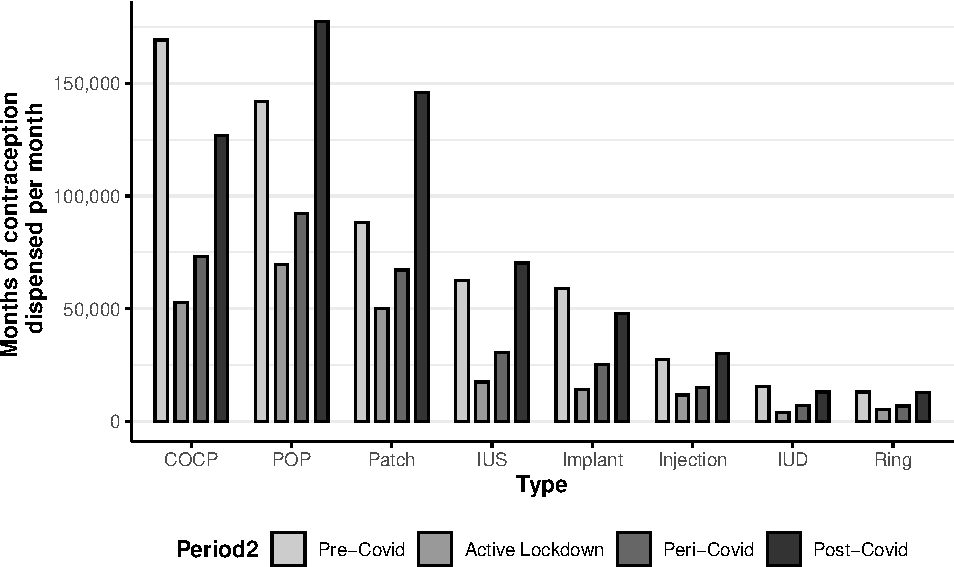
\includegraphics{Manuscript_files/figure-latex/Figure1-1.pdf}
\caption{Covid-19 restrictions changed the proportions of categories of
contraception dispensed in Scotland. Prior to Covid-19, the combined
oral contraceptive pill (COCP), containing both osetrogens and
progesterones was the most dispensed form of contraception. However,
during the Covid-19 pandemic, this changed to the progesterone-only pill
(POP), with dispensing of the contraceptive patch also increasing.
Dispensing rates of long-acting reversible contraception (LARC)
including the IUS, IUD, injection and implant decreased during Covid-19,
whilst the contraceptive ring remained relatively stable.}
\end{figure}

Periods of active lockdown resulted in large decreases in all forms of
contraception being dispensed in Scotland (Table 3).

\begin{longtable}{lrrrrrrrrrrrrrr}
\toprule
 & \multicolumn{5}{c}{LARCs} & \multicolumn{3}{c}{Oral} & \multicolumn{3}{c}{Other} & \multicolumn{3}{c}{EC} \\ 
\cmidrule(lr){2-6} \cmidrule(lr){7-9} \cmidrule(lr){10-12} \cmidrule(lr){13-15}
Timeframes & All LARC & IUS & IUD & Implant & Injection & All Oral & COCP & POP & All Other & Patch & Ring & All EC & Uli & Levo \\ 
\midrule
Lockdown & $28.89\%$ & $28.02\%$ & $25.38\%$ & $24.32\%$ & $42.69\%$ & $39.37\%$ & $31.30\%$ & $49.00\%$ & $54.64\%$ & $56.61\%$ & $41.40\%$ & $37.62\%$ & $86.54\%$ & $26.54\%$ \\ 
Peri-Lockdown & $47.31\%$ & $48.89\%$ & $44.55\%$ & $42.86\%$ & $54.85\%$ & $53.17\%$ & $43.32\%$ & $64.92\%$ & $72.99\%$ & $76.03\%$ & $52.58\%$ & $60.87\%$ & $141.99\%$ & $42.48\%$ \\ 
Post-Lockdown & $98.08\%$ & $112.54\%$ & $83.63\%$ & $81.10\%$ & $109.91\%$ & $97.86\%$ & $75.04\%$ & $125.07\%$ & $156.45\%$ & $165.09\%$ & $98.43\%$ & $121.11\%$ & $357.97\%$ & $67.42\%$ \\ 
\bottomrule
\end{longtable}

\hypertarget{oral-contraception}{%
\subsection{Oral contraception}\label{oral-contraception}}

Oral contraceptives comprising of both COCP and POP were consistently
the most prescribed form of contraception in Scotland, as measured by
both months of contraceptive coverage dispensed per month, and the total
number of items dispensed.

Prior to the Covid-19 pandemic, combined oral contraceptives were more
frequently prescribed (mean percentage of total months of contraception
dispensed per month 54.38\%) than progesterone-only contraceptives
(45.62\%). However, during the period from April 2020 to April 2022,
this trend was reversed (COCP: 43.84\%, POP: 56.16\%). Restrictions on
face-to-face medical appointments during Covid-19 meant that the regular
monitoring of BMI, and blood pressure were unable to take place. This
likely lead to the decrease in COCP prescribing, and the growth in
dispensing of POPs instead (Figure 2), which do not require the same
patient monitoring.After this period, the trend has not restored to
pre-Covid-19 levels, but in fact the dispensing of POP have increased
(COCP: 41.70\%, POP: 58.30\%). Intriguingly, the differences in the
proportion of COCP versus POP dispensed per month in Scotland have
widened even after the lifting of Covid-19 associated restrictions
(Figure 2).

\begin{figure}
\centering
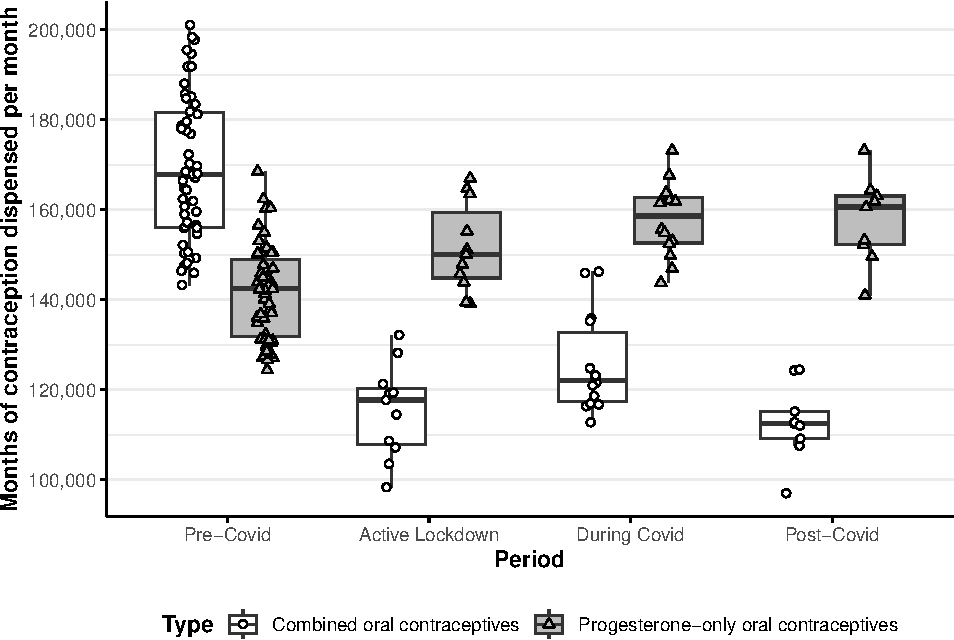
\includegraphics{Manuscript_files/figure-latex/Figure2-1.pdf}
\caption{Testing}
\end{figure}

However, some of this variation may be due to a decline in the total
months of contraceptive coverage dispensed. During Covid-19, a mean of
287,775 MCC were dispensed per month, a 7.45\% reduction in MCC
dispensed per month compared with pre-Covid-19 levels (310,952). This
trend has abated post-Covid-19, but the level of MCC dispensed per month
remains 2.14\% below pre-Covid-19 levels (304,309).

\hypertarget{long-acting-reversible-contraception}{%
\subsection{Long-acting reversible
contraception}\label{long-acting-reversible-contraception}}

Long-acting reversible contraception (LARC), generally requires
administration by a healthcare professional, unlike oral contraception.
Due to the aforementioned restrictions on face-to-face appointments,
LARC administration was severely decreased throughout the Covid-19
pandemic (Figure 3).

The decrease in injection dispensing throughout Covid-19 is less severe
than other forms of LARC which cannot be self-administered. There was a
change in dispensing type, with Depo-Provera (IM) decreasing to 75.64\%
of pre-pandemic levels during periods of lockdown, and Sayana Press (SC)
increasing to 111.04\%.

\begin{figure}
\centering
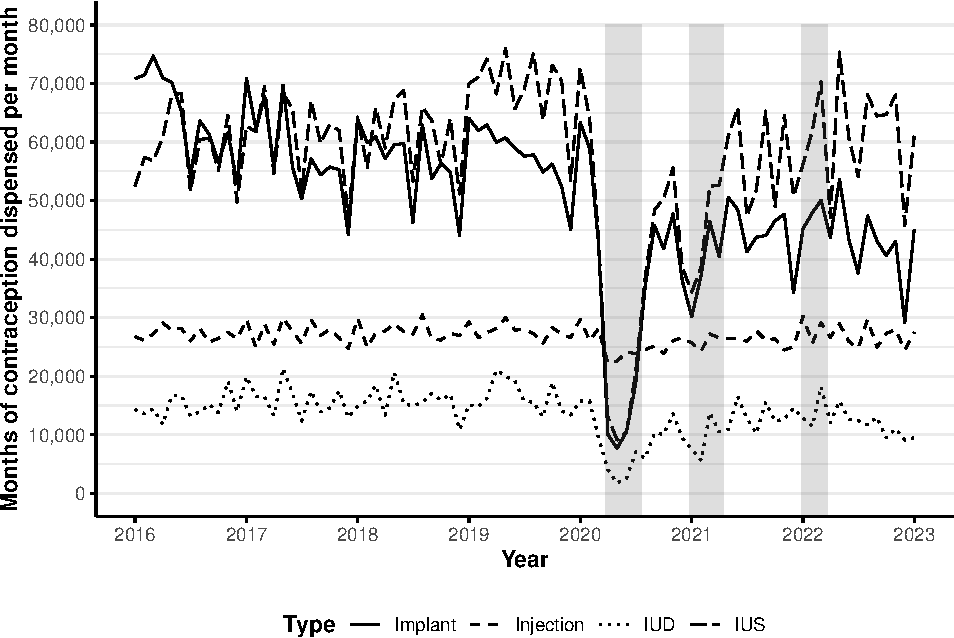
\includegraphics{Manuscript_files/figure-latex/Figure3-1.pdf}
\caption{Grey shaded areas indicate active lockdowns.}
\end{figure}

\hypertarget{emergency-contraception}{%
\subsection{Emergency contraception}\label{emergency-contraception}}

Emergency contraception is available free-of-charge without a
prescription from the majority of Scottish community pharmacies
(MacCrimmon 2015). Due to social restrictions present in Scotland, it
was expected to see a decrease in emergency contraception dispensing
(Figure 4).

\begin{figure}
\centering
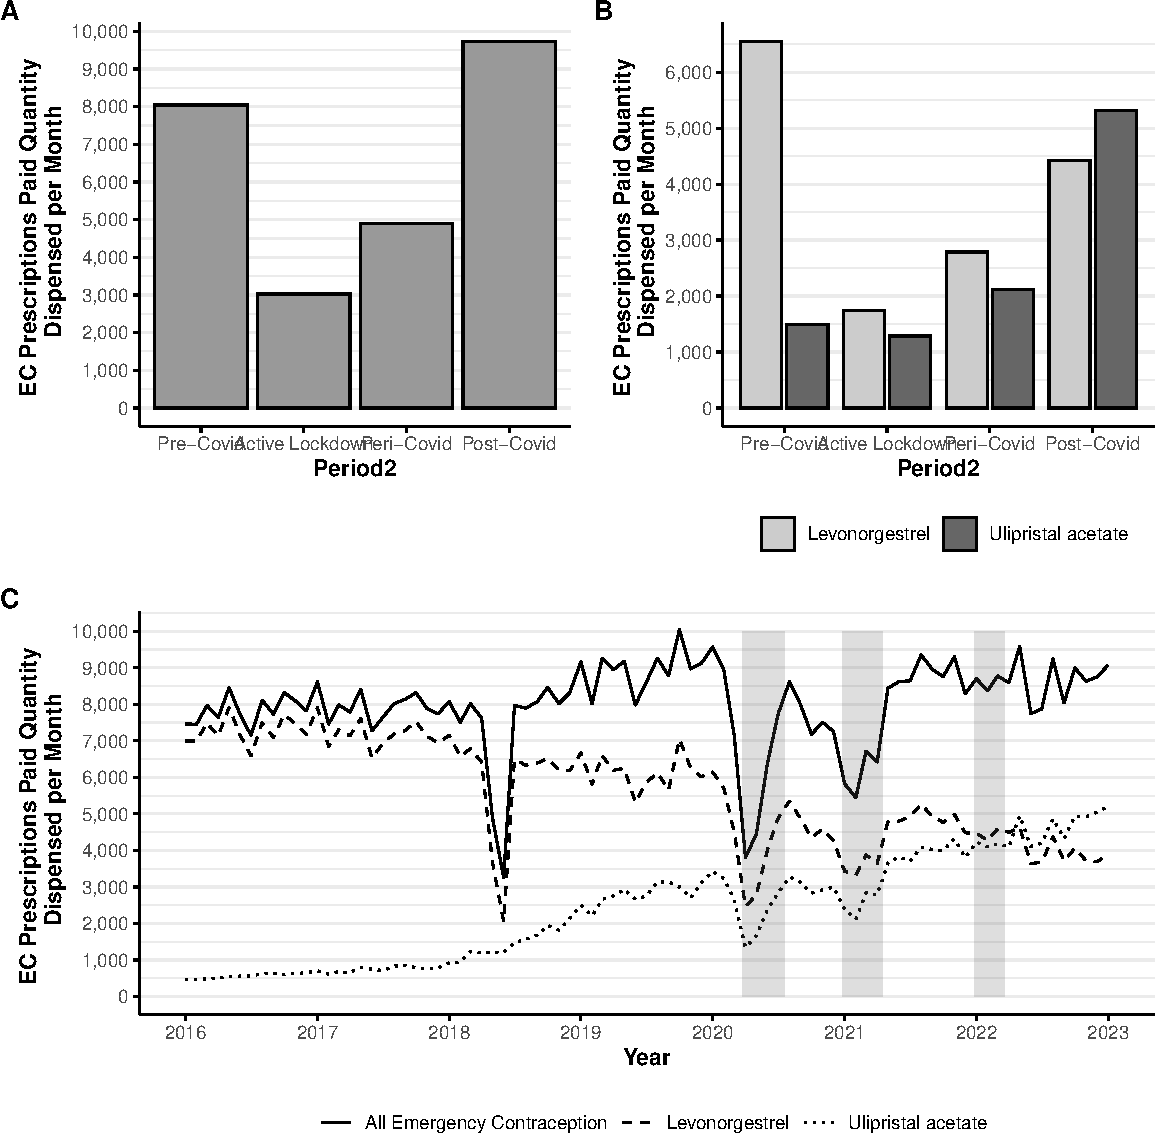
\includegraphics{Manuscript_files/figure-latex/Figure4-1.pdf}
\caption{Emergency contraception}
\end{figure}

\hypertarget{discussion}{%
\section{Discussion}\label{discussion}}

The clear decreases in all forms of prescribed contraceptive provision
in Scotland during Covid-19 presents a myriad of possible outcomes
ranging from unwanted pregnancies to

Telemedicine terminations, easier to access and potentially increased
due to this lack of effective contraceptive provision for Scottish
women.

FRSH

The effects of these restrictions appear to have altered trends in
contraceptive prescribing within Scottish general practice. For example,
the increasing role of progeterone-only oral contraception are clerarly
visible. This is also supported by access to POPs within community
pharmacies in Scotland.

\hypertarget{limitations}{%
\subsection{Limitations}\label{limitations}}

Assumption that any changes observed between 2016 etc are due to
lockdown and other restrictions, not due to other unknown factors.

A further assumption is made that the patient population seeking
contraception from general practioners is constant throughout the period
of this study, and consequently, variances in prescribing rates between
pre and post covid are due to changes in contraceptive prescribing
rather than population level alterations.

Finally, it also assumed that the drugs dispesed here are used purely
for their licenced indication of contraception, not any alternative eg
HRT or off-label uses.

Only data from Scotland were included in this study. Future work may
explore if these impacts were similar in the other nations of the UK, or
whether the devolved nature of healthcare policy within the UK created
disparities in access to contracpetion during Covid-19 restrictions.

\hypertarget{conclusions}{%
\section{Conclusions}\label{conclusions}}

\hypertarget{reference-list}{%
\section{Reference List}\label{reference-list}}

\hypertarget{refs}{}
\begin{CSLReferences}{1}{0}
\leavevmode\vadjust pre{\hypertarget{ref-BNF2023}{}}%
Joint Formulary Committee. 2023. \emph{British National Formulary
(Online)}. London: BMJ; Pharmaceutical Press.
\url{https://bnf.nice.org.uk}.

\leavevmode\vadjust pre{\hypertarget{ref-EHC2015}{}}%
MacCrimmon, Suzanne. 2015. \emph{Emergency Hormonal Contraception (EHC)
Service Service Specification}. Edinburgh, Scotland: Community Pharmacy
Scotland.
\url{https://members.cps.scot/media/e5fbbpn3/109813-ehcservicespec_17sep2015.pdf}.

\leavevmode\vadjust pre{\hypertarget{ref-RCoreTeam2021}{}}%
R Core Team. 2023. \emph{R V4.3.0: A Language and Environment for
Statistical Computing}. Vienna, Austria: R Foundation for Statistical
Computing. \url{https://www.R-project.org/}.

\leavevmode\vadjust pre{\hypertarget{ref-Walker2022}{}}%
Walker, Susan H. 2022. {``Effect of the COVID-19 Pandemic on
Contraceptive Prescribing in General Practice: A Retrospective Analysis
of English Prescribing Data Between 2019 and 2020.''}
\emph{Contraception and Reproductive Medicine} 7 (1): 3.
\url{https://doi.org/10.1186/s40834-022-00169-w}.

\end{CSLReferences}

\hypertarget{supporting-information}{%
\section{Supporting information}\label{supporting-information}}

\end{document}
